\graphicspath{{Kapitel/Kapitel4_Hauptteil/Images/}}

Dieses Kapitel beschreibt die Virtual Reality Applikation \textbf{C.LABEL-VR} und ist somit der Hauptteil dieser Arbeit. Das Ziel dieser Applikation ist es die Annotierung von Punktwolken, wie sie beispielsweise in \textbf{C.LABEL}(siehe Kapitel \ref{sec:C.LABEL}) möglich ist, innerhalb einer dreidimensionalen Umgebung zu realisieren. Dazu müssen Datenformate, welche Informationen über Punktwolken enthalten, eingelesen und anschließend, aus diesen Daten, Punktwolken generiert werden. Der Vorgang des Imports wird in Kapitel \ref{sec:ImportExport} näher beschrieben, die Generierung der Punktwolken in \ref{sec:Generierung}. Um sich in der virtuellen Umgebung durch diese Wolken bewegen zu können, wurden diverse Möglichkeiten zur Navigation entwickelt. Auf die Funktion dieser Möglichkeiten und deren Auswirkungen auf das befinden des Menschen (\textit{Virtual Motion Sickness}) wird in Kapitel \ref{sec:Navigation} eingegangen. 

Anschließend geht es um die Annotierung der generierten Punktwolken. Annotierung bedeutet in diesem Kontext, dass die einzelnen Punkte der Wolken mit bestimmten Klassifikationen versehen werden, welche der Art des Objektes entsprechen, dem die Punkte zugehören. Ist der Punkt beispielsweise Bestandteil eines Autos, so wird er mit der Klasse \glqq Auto\grqq{} versehen. Um diese Aufgabe erfüllen zu können wurden mehrere Arten der Annotierung entwickelt. Welche dies sind und wie sie realisiert wurden, wird in Kapitel \ref{sec:Annotation} gezeigt. Das letzte Kapitel \ref{sec:UIMenu} beschäftigt sich mit dem User Interface der Applikation. Dabei wird hauptsächlich auf die Funktionen des Ingame-Menüs eingegangen, welche Herausforderungen es bei der Erstellung von \acrshort{acr:UI}s in der virtuellen Realität gibt und wie diese bewältigt wurden. Zur Veranschaulichung der Funktionen von \textbf{C.LABEL-VR} ist in der Abbildung \ref{fig:Workflow} der grobe \gls{glos:Workflow} in Form eines Diagramms abgebildet.

\begin{figure}%
	\centering
    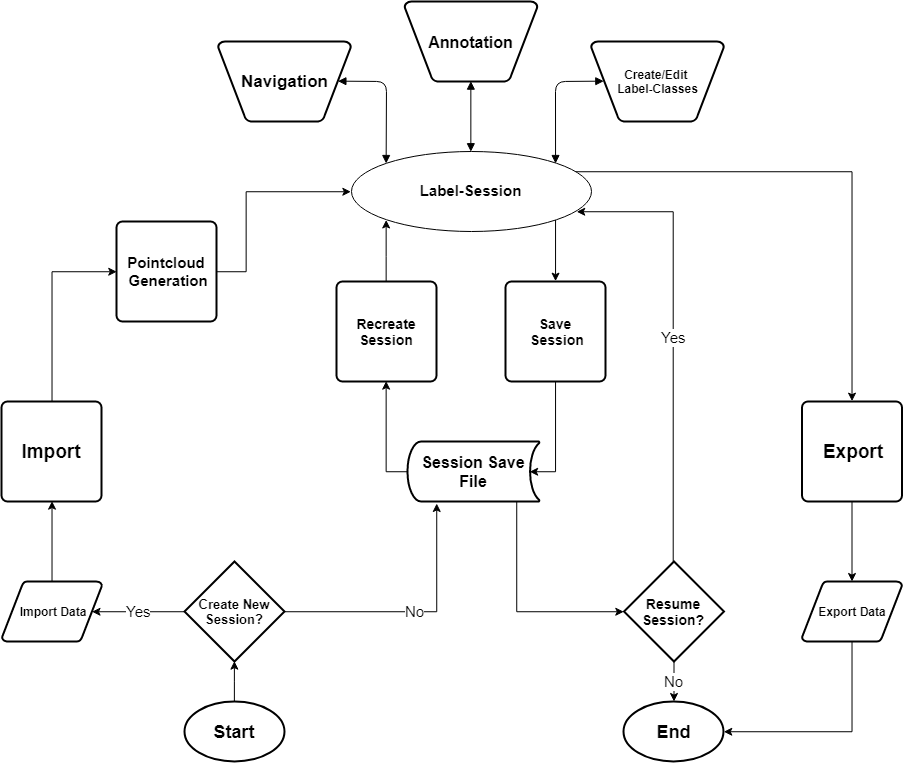
\includegraphics[width=13.5cm]{Workflow}
    \caption{\glslink{glos:Workflow} in C.LABEL-VR vom Import bis zum Export}
    \label{fig:Workflow}
\end{figure}

\section{Import und Export von Daten}
\label{sec:ImportExport}
Umfeldmodelle, welche in Form einer Punktwolke vorliegen, werden meist von einem Radar-, oder, wie in Kapitel \ref{sec:Lidar} gezeigt, von einem Lidar-Sesnor aufgenommen. Die Informationen über diese Modelle, zum Beispiel die Positionen der einzelnen Punkte, werden in einem passenden Datenformat abgespeichert. Um welches Format es sich dabei handelt kann sehr unterschiedlich sein. In der Regel hängt es davon ab zu welchem Zweck die aufgenommenen Daten gebraucht werden und wie umfangreich diese Daten sind. Am häufigsten werden sie dafür verwendet um Lernalgorithmen und neuronale Netze (siehe \ref{sec:KNN}) zu trainieren. Automobilhersteller haben für solche Vorhaben natürlich unterschiedliche Konzepte und somit können auch die Formate der Daten unterschiedlich sein. Um die Applikation \textbf{C.LABEL-VR} für mehrere dieser Hersteller benutzbar zu machen, muss das Programm also mit verschiedenen Datenformaten umgehen können.\\ 

Innerhalb dieser Arbeit wurden mit zwei verschiedenen Arten von Daten gearbeitet. Das erste Format ist das \textbf{PCD}-Format (\textit{Point Cloud Data}). Die \gls{glos:OpenSrc}-Bibliothek \textbf{PCL}(\textit{Point Cloud Library}) benutzt das Datenformat \textbf{PCD} um Informationen über Punktwolken zu verwalten. \textbf{PCL} ist eine sehr mächtige C++-Bibliothek, die in der Regel von jedem benutzt wird, der performante Algorithmen für Punktwolken entwickeln möchte. Auch \textbf{C.LABEL} (siehe \ref{sec:C.LABEL}) generiert aus eingelesenen Daten \textbf{PCD}-Files um Funktionen der Point Cloud Library für die Wolken zu benutzen.

Das zweite Format ist das, von der HDF-Group bereitgestellte, \textbf{HDF5}-Format (\textit{Heterogeneous Data Format}). Es ist ausgelegt zum schnellen Erstellen und Auslesen von komplexen und großen Datenstrukturen. Welche Elemente diese Strukturen enthalten können wird später in Kapitel \ref{sec:HDF5} erklärt. Zur schnellen Bearbeitung großer Datenmengen ist dies ein gängiges Format und wird von den meisten Kunden von \textbf{CMORE} benutzt um Sensordaten zu verwalten. Deshalb wird es auch in \textbf{C.LABEL-VR} verwendet.\\

\subsection{Architektur}

Wichtig ist es also sowohl den Import, als auch den Export so modular wie möglich zu gestalten, dass \textbf{C.LABEL-VR} ohne große Änderungen  an der Hauptapplikation um neue Datenformate erweitert werden kann. Das Prinzip  dafür ist in Abbildung \ref{fig:ImportExport} dargestellt und wird im Folgenden näher erläutert. Die angesprochenen Erweiterungen um neue Datenformate werden als \textit{Addons} bezeichnet. Jedoch handelt es sich dabei nicht immer nur um eine Erweiterung eines, von Grund auf, neuen Datenformates. Komplexe Formate, wie zum Beispiel \textbf{HDF5}, in denen der Entwickler die Struktur selbst festlegt, müssen für jede neue Struktur, auf unterschiedliche Weise eingelesen werden und brauchen somit auch separate \textit{Addons}. Um die Erweiterbarkeit der Applikation sicherzustellen wurde der Import und der Export von der Hauptapplikation \glqq abgekapselt\grqq . Dafür wurde eine interne Datenstruktur (kurz \acrshort{acr:IDS}) eingeführt, welche alle nötigen Informationen enthält, die für das \glslink{glos:Labeling}{Labeling} notwendig sind. Sie wird im späteren Kapitel \ref{sec:IDS} genauer vorgestellt. Der Vorteil dabei ist, dass die Hauptapplikation dadurch stets auf die gleiche Datenstruktur zurückgreifen kann und somit unabhängig vom importierten Datenformat ist. Wird also ein neues Import-Format eingeführt muss an der Hauptapplikation nichts verändert werden. \\ 

Jedes Import-\textit{Addon} hat also zunächst die Aufgabe, seine jeweiligen Daten einzulesen und alle Informationen, die für die \acrshort{acr:IDS} notwendig sind, daraus zu extrahieren. Aus diesen Informationen können anschließend die entsprechenden Punktwolken generiert werden. Die Generierung wird in Kapitel \ref{sec:PclGenerate} erklärt. Beim Export ist es notwendig, dass die Struktur der, vom Import-\textit{Addon} eingelesenen, Daten gleich bleibt. Es sollen lediglich die \glslink{glos:Labeling}{Labeling}-Informationen aus der \acrshort{acr:IDS} hinzu- bzw. eingefügt werden. Aus der \acrshort{acr:IDS} kann das Export-Addon diese Informationen extrahieren und anschließend in die eingelesenen Daten exportieren. Die importierten Daten werden so allerdings überschrieben. Möchte man das nicht, müssen die Daten neu erstellt und mit den \glslink{glos:Labeling}{Labeling}-Informationen versehen werden. \\

Die Importierten Daten, beispielsweise \textbf{HDF5}, enthalten allerdings oft deutlich mehr Informationen, als für die interne Struktur notwendig. Diese Zusatzinformationen werden \textit{Metadaten} genannt. Für den Export bedeutet dies, dass man aus der internen Datenstruktur von \textbf{C.LABEL-VR}, die Struktur der anfangs eingelesenen Daten nicht wieder rekonstruieren kann, da die \textit{Metadaten} fehlen würden. Um dieses Problem zu lösen müssen die zusätzlichen Daten separat gespeichert werden. Dazu wurde eine erweiterbare Datenstruktur angelegt, in der man für jede Import-Struktur eine Metadatenstruktur anlegen kann. Das entsprechende Export-Addon kann die Metadaten dann verwenden um, zusammen mit den internen Daten, das gewünschte Exportformat zu rekonstruieren. \\

\begin{figure}%
	\centering
    \includegraphics[width=13.5cm]{Import_Export_Architecture}
    \caption{Das Import-Export-Prinzip in C.LABEL-VR}
    \label{fig:ImportExport}
\end{figure}

Zusammenfassend ist also folgendes zu tun um die Benutzung ein neues Datenformates oder einer neuen Datenstruktur zu gewährleisten: Zunächst muss eine Importfunktion programmiert werden, die alle Informationen aus den gewünschten Daten ausliest. Anschließend muss diese Funktion das genormte, interne Datenformat (Kapitel \ref{sec:IDS}) erstellen und alle nötigen Informationen aus den eingelesenen Daten darin speichern, damit daraus die entsprechenden Punktwolken generiert werden können. Falls es Daten gibt, die über diejenigen in der \acrshort{acr:IDS} hinausgehen, muss eine Metadatenstruktur angelegt werden, in welche die zusätzlichen Daten abgelegt werden können. Zuletzt ist eine Exportfunktion zu implementieren, die sowohl die \glslink{glos:Labeling}{Labeling}-Informationen aus der \acrshort{acr:IDS} in die eingelesenen Daten exportieren kann, als auch aus den internen- und den Metadaten das Ausgangsdatenformat wiederherstellen kann, um die Daten als neue Files zu exportieren. Im folgenden Kapitel soll dieses Prinzip konkret an einem HDF5-Beispiel gezeigt werden.

\subsection{HDF5-Beispiel}
\subsubsection{HDF5 Daten}
\label{sec:HDF5}
\subsubsection{Beispiel}

\section{Generierung einer Punktwolke}
\label{sec:Generierung}

\subsection{Interne Datenstruktur}
\label{sec:IDS}

\subsection{Generierung}
\label{sec:PclGenerate}
session
pointcloud
...

Koordinatensysteme

\subsection{Optimierung}
-generell nichts teures in update mehthode
	
-gameobject find
-getcomponent

keine update oder start mehtode bei skripten der punkte
collider trigger nicht bei den punkten sondern beim anderen object
generell alle pollenden aktionen von den punkten entfernen


(-clonen von prefabs statt neue instanzen von inbuilts)
shared materials verwenden   kein material.color weil das eine kopie des materials erzeugt, welches dann einzeln gecallt werden muss

gpu instancing bei den materials verwenden und forward rendering options

\section{Navigation}
\label{sec:Navigation}
\subsection{VR-Krankheit}
\subsection{Freier Flug}
\subsection{Teleport}

\section{Annotieren der Punktwolke}
\label{sec:Annotation}
\subsection{Pointer Labeling}
\subsection{Clustering}
\subsubsection{ground plane fitting}
%https://en.wikipedia.org/wiki/Singular-value_decomposition
%https://www.ltu.se/cms_fs/1.51590!/svd-fitting.pdf

\section{Ingame Menu}
\label{sec:UIMenu}
\subsection{Movement}
\subsection{Labelclasses}


